\chapter{Troubleshooting}\label{cha:Troubleshooting}


\section*{FAQ}
\begin{description}
\item [{configuration fails:}]~


Examine the log file 'config.log'. It contains detailed informations.
In many cases, the paths to these specific compiler commands F90,
CC and MPIF90 will not be correct if `./configure` fails.


Please make sure that you have a working installation of a Fortran
compiler, a C compiler and an MPI implementation. You should be able
to compile this little program code:

{\footnotesize
\begin{verbatim}
 program main
 include 'mpif.h'
 integer, parameter :: CUSTOM_MPI_TYPE = MPI_REAL
 integer ier
 call MPI_INIT(ier)
 call MPI_BARRIER(MPI_COMM_WORLD,ier)
 call MPI_FINALIZE(ier)
 end
\end{verbatim}
}

\item [{compilation fails stating:}] ~
{\footnotesize
\begin{verbatim}
...
 obj/program_generate_databases.o: In function `MAIN__':
 program_generate_databases.f90:(.text+0x14): undefined reference to `_gfortran_set_std'
...
\end{verbatim}
}

Make sure you're pointing to the right 'mpif90' wrapper command.


Normally, this message will appear when you are mixing two different
Fortran compilers. That is, using e.g. gfortran to compile non-MPI
files and mpif90, wrapper provided for e.g. ifort, to compile MPI-files.


fix: e.g. specify > ./configure FC=gfortran MPIF90=/usr/local/openmpi-gfortran/bin/mpif90

\item [{after executing \texttt{xmeshfem3D} I've got elements with skewness of 81\% percent, what does this mean:}] Look
at the skewness table printed in the \texttt{output\_mesher.txt} file
after executing \texttt{xmeshfem3D} for the example given in \texttt{EXAMPLES/meshfem3D\_examples/simple\_model/}:

{\footnotesize
\begin{verbatim}
...
 histogram of skewness (0. good - 1. bad):
 0.0000000E+00 - 5.0000001E-02 27648 81.81818 %
 5.0000001E-02 - 0.1000000 0 0.0000000E+00 %
...
\end{verbatim}
}

The first line means that you have 27,648 elements with a skewness
value between 0 and 0.05 (which means the element is basically not
skewed, just plain regular hexahedral element). The total number of
elements you have in this mesh is (see in the \texttt{output\_mesher.txt}
file a bit further down):

{\footnotesize
\begin{verbatim}
...
 total number of elements in entire mesh: 33792
...
\end{verbatim}
}

which gives you that: 27,648 / 33,792 $\sim$ 81.8 \% of all elements
are not skewed, i.e. regular elements. a fantastic value :)


The histogram lists for this mesh also some stronger skewed elements,
for example the worst ones belong to:

{\footnotesize
\begin{verbatim}
...
 0.6000000 - 0.6500000 2048 6.060606 %
...

\end{verbatim}
}

about 6 \% of all elements have distortions with a skewness value
between 0.6 and 0.65. The skewness values give you a hint of how good
your mesh is. In an ideal world, you would want to have no distortions,
just like the 81\% from above. Those elements give you the best approximate
values by the GLL quadrature used in the spectral-element method.
However, having weakly distorted elements is still fine and the solutions
are still accurate enough. So empirically, values up to around 0.7
are tolerable, above that you should consider remeshing...


To give you an idea why some of the elements are distorted, see the
following figure \ref{fig:mesh.vp} of the mesh you obtain in the
example \texttt{EXAMPLES/meshfem3D\_examples/simple\_model/}.
\begin{figure}[htbp]
\noindent \begin{centering}
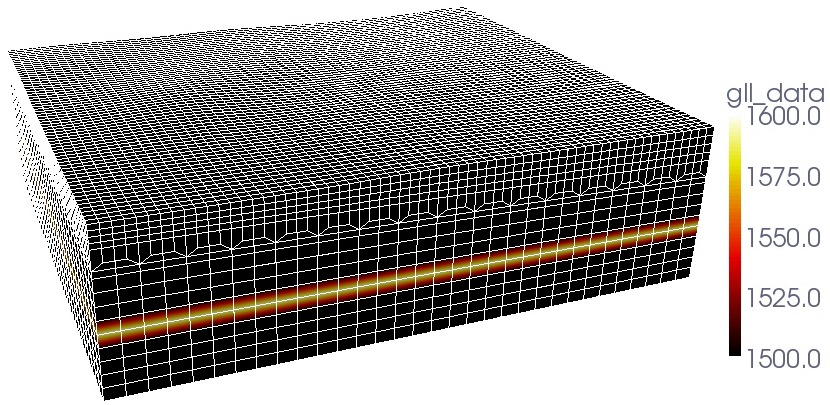
\includegraphics[width=0.9\textwidth]{figures/mesh_vp.jpg}
\par\end{centering}

\caption{Paraview visualization using the mesh vtk-files for the example given
in \texttt{EXAMPLES/meshfem3D\_examples/simple\_model/}.}


\label{fig:mesh.vp}
\end{figure}



You will see that the mesh contains a doubling layer, where we stitch
elements together such that the size of two elements will transition
to the size of one element (very useful to keep the ratio of wavespeed
/ element\_size about constant). Those elements in this doubling layer
have higher skewness values and make up those 6 \% in the histogram.

\item [{the code gives following error message "need at least one receiver":}] This
means that no stations given in the input file \texttt{DATA/STATIONS}
could be located within the dimensions of the mesh. This can happen
for example when the mesh was created with the in-house mesher \texttt{xmeshfem3D}
while using the Universal Transverse Mercator (UTM) projection but
the simulation with \texttt{xspecfem3D} was suppressing this projection
from latitude/longitude to x/y/z coordinates.


In such cases, try to change your \texttt{DATA/Par\_file} and set
e.g.:
\begin{verbatim}
SUPPRESS_UTM_PROJECTION = .false.
\end{verbatim}
to be the same in \texttt{Mesh\_Par\_file} and \texttt{Par\_file}.
This flag should be identical when using the in-house mesher \texttt{xmeshfem3D},
\texttt{xgenerate\_databases} and \texttt{xspecfem3D} together to
run simulations.


The flag determines if the coordinates you specify for your source
and station locations are given as lat/lon degrees and must be converted
to UTM coordinates. As an example, if you use \texttt{.false.} within
\texttt{Mesh\_Par\_file} then you create a mesh with \texttt{xmeshfem3D}
using the UTM projection from lat/lon as input format to UTM projected
coordinates to store the mesh point positions, which is fine. The
error then may occur if in the \texttt{Par\_file} you have this set
to \texttt{.true.} so that the \texttt{xgenerate\_databases} and \texttt{xspecfem3D}
suppress the UTM projection and assume that all coordinates you use
now for source and receiver locations are given in meters (that is,
converted) already. So it won't find the specified locations in the
used mesh. As a solutions, just change the flag in \texttt{Par\_file}
to be the same as in \texttt{Mesh\_Par\_file} and rerun \texttt{xgenerate\_databases}
and \texttt{xspecfem3D} to make sure that your simulation works fine.

\item [{I get the following error message "forward simulation became unstable and blew up":}] In
most cases this means that your time step size \texttt{DT} is chosen
too big. Look at your files \texttt{output\_mesher.txt} or \texttt{output\_solver.txt}
created in the folder \texttt{OUTPUT\_FILES}. In these output files,
find the section:

{\footnotesize
\begin{verbatim}
...
 *********************************************
 *** Verification of simulation parameters ***
 *********************************************
...
 *** Minimum period resolved = 4.308774
 *** Maximum suggested time step = 6.8863556E-02
...
\end{verbatim}
}

then change \texttt{DT} in the \texttt{DATA/Par\_file} to be somewhere
close to the maximum suggested time step. In the example above: \\
 \texttt{DT = 0.05d0} \\
 would (most probably) work fine. It could be also bigger than the
0.068 s suggested. This depends a bit on the distortions of your mesh
elements. The more regular they are, the bigger you can choose \texttt{DT}.
Just play with this value a bit and see when the simulation becomes
stable ...

\end{description}

